\chapter{Аналитический раздел}
\label{cha:analysis}
\section{Анализ предметной области}
Сегодня невозможно представить человека без интернета и информационных технологий. Они прочно вошли в нашу жизнь, значительно упростив ее. С развитием информационных технологий нам становятся доступны новые инструменты, которые делают привычные нам процессы удобнее и быстрее, например: покупка товаров, оплата счетов, развлечения и многое другое. Наблюдается стремительный рост пользователей сети Интернет и объемов информации. Такое стремительное развитие в первую очередь отражается на интернет-провайдерах.

На рисунке~\ref{pic:user_connection_schema} представлена стандартная схема подключения пользователей к сети провайдера.
\begin{figure}
\centering
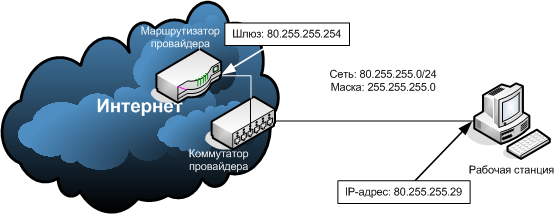
\includegraphics[scale=0.7]{pictures/user_connection_schema}
\caption{Подключение пользователя к сети Интернет}
\label{pic:user_connection_schema}
\end{figure}

В зависимости от видов предоставляемых услуг провайдеры делятся на:
\begin{itemize}
\item провайдеры доступа;
\item хостинг-провайдеры;
\item магистральные провайдеры;
\item канальные провайдеры;
\item провайдеры последней мили;
\end{itemize}

Независимо от того, к какой категории относятся провайдеры, они должны обеспечивать бесперебойную, надежную и высокоскоростную передачу данных абонентам. Данные задачи решаются такими методами, как:
\begin{itemize}
\item дублирование информации с целью минимизации расстояния между источником и потребителем;
\item увеличение пропускной способности каналов передачи данных;
\item приоритизация трафика и динамическое управление;
\end{itemize}

Подход, связанный с дублированием (репликацией) информации, активно используется на серверах баз данных. Является дорогим, так как требует дополнительных финансовых расходов, связанных с закупкой оборудования для хранения копий. Также требуется постоянная синхронизация между копиями для достижения консистентности данных.

Второй подход также связан с изменение сетевой инфраструктуры - модернизация каналов передачи данных с целью увеличения пропускной способности. Достигается за счет использования более быстрых способов коммутации, например оптоволокно. Аналогично первому подходу является дорогим.

Данная работа посвящена третьему подходу, связанному с приоритизацией и динамическим управлением трафиком. Основная идея заключается в классификации трафика по каким-то критериям и обработке разными способами. На рисунке \ref{pic:qos_simple_example} приведен пример использования классификации трафика для реализации QoS. Маршрутизатор 1 настроен таким образом, чтобы выделить до 5 МБит/с из доступных 10 МБит/с передаче потокового видео. Передаче данных по FTP разрешено использовать 2МБит/с, а HTTP и другому трафику до 3 МБит/с.
\begin{figure}
\centering
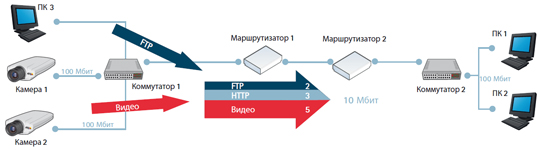
\includegraphics[scale=0.7]{pictures/qos_simple_example}
\caption{Пример динамического управления трафиком}
\label{pic:qos_simple_example}
\end{figure}

\subsection{Сетевая модель OSI и стек протоколов TCP/IP}
Сетевая модель OSI - базовая эталонная модель взаимодействия открытых систем. Назначение модели OSI состоит в обобщенном представлении средств сетевого взаимодействия, она разрабатывалась в качестве универсального языка сетевых специалистов, поэтому ее называют справочной моделью.

В связи с затянувшейся разработкой протоколов OSI, в настоящее время основным стеком протоколов является TCP/IP~\cite{modern_net}. Протоколы работают друг с другом в стеке - это означает, что протокол, располагающийся на уровне выше, работает
"поверх" нижнего, используя механизмы инкапсуляции. На рисунке~\ref{pic:model_osi_vs_tcpip} приведены обе модели, а также показаны их основные различия.
\begin{figure}[h]
\centering
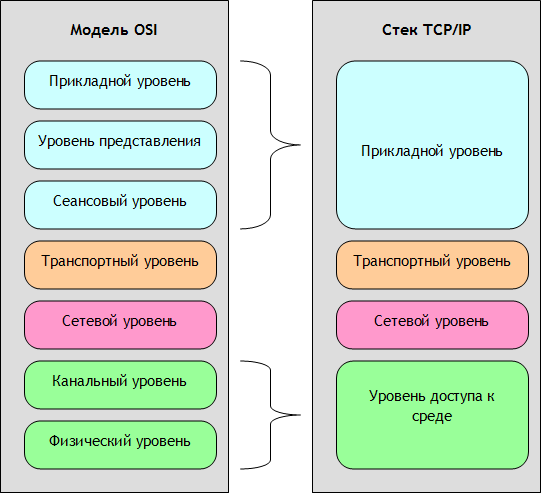
\includegraphics[scale=0.5]{pictures/model_osi_vs_tcpip}
\caption{Модель OSI и TCP/IP}
\label{pic:model_osi_vs_tcpip}
\end{figure}

На канальном уровне в большинстве сетей используется семейство технологий пакетной передачи данных Ethernet. В зависимости от скорости передачи данных, а также передающей среды, существует несколько вариантов технологии:
\begin{itemize}
\item ранние модификации Ethernet;
\item 10 МБит/с Ethernet;
\item Быстрый Ethernet (Fast Ethernet, 100 МБит/с);
\item Гигабитный Ethernet (Gigabit Ethernet, 1 ГБит/с);
\item 2.5 и 5-гигабитные варианты (NBASE-T, MGBASE-T);
\item 10-гигабитный Ethernet (10G Ethernet, 10 ГБит/с);
\item 40-гигабитный и 100-гигабитный Ethernet;
\end{itemize}

Разрабатываемый сетевой сервис будет работать только с Ethernet картами любых скоростей, при этом другие технологии канального уровня не поддерживаются.

\subsection{Технология DPI}
Анализ пакетов является важной задачей не только для классификации трафика, но и для всего функционирования сети. Любой сетевой коммутатор вынужден просматривать каждый пакет с целью изучения его mac-адреса отправителя и получателя. Эта информация нужна ему для того, что определить в какой выходной порт отправить пакет. Сетевые маршрутизаторы просматривают ip-адреса отправителя и получателя (если речь идет о TCP/IP сетях) и строят таблицы маршрутизации.

В наше время провайдеры сталкиваются с проблемами, которые не могут решиться только анализом заголовков пакетов, например:
\begin{itemize}
\item высокая загрузка канала к пользователю (скачивание BitTorrent);
\item высокая нагрузка на каналы провайдера (все пользователи скачивают BitTorrent);
\item большая часть пропускной способности занимается наименьшей частью наиболее активных абонентов;
\item атаки на оборудование, вирусы, боты;
\end{itemize}

Для решения всех этих проблем может применяться технология DPI - технология накопления статистических данных, проверки и фильтрации сетевых пакетов по их содержимому. Ключевая идея состоит в том, чтобы анализировать не только заголовки пакетов, такие как Ethernet, IP, TCP или UDP, но и остальные данные пакета с целью выявления определенных сигнатур или других особенностей, присущих искомому трафику. Самыми распространенными способами реализации DPI являются статический анализ и анализ косвенных признаков, присущих определенным протоколам. 

Система DPI, как правило, устанавливается на границе сети провайдера в разрыв существующих каналов, уходящих в пограничные маршрутизаторы, тем самым весь трафик, который покидает или входит в сеть оператора проходит через DPI, что дает возможность его мониторинга и контроля. В отдельных случаях можно устанавливать эту систему не на границе сети, а спускать ее ближе к конечным пользователям, но из экономических соображений так делают редко.

На рынке DPI есть модели от различных вендоров по различным ценам, все зависит от производительности и списка возможностей. В данной работе рассматривается чисто программная реализация технологии DPI под архитектуру процессоров x86\_64.


\section{QoS и DPI}
С точки зрения эксплуатации, провайдер может контролировать утилизацию подключенных через DPI каналов на уровне приложений. Раньше задача реализации QoS решалась исключительно средствами построения очередей на основании маркировки трафика служебными битами в заголовках IP, а также используя VLAN или MPLS метки, выделяя наиболее приоритетный трафик и гарантируя ему определенную пропускную способность в любой момент времени. При этом весь трафик домашних абонентов оставался без контроля, что давало возможность трафику BitTorrent забрать себе всю свободную полосу.

С использованием DPI у провайдера появляется возможность распределить канал между различными приложениями, так, например, можно разрешить в ночные часы BitTorrent с большей пропускной способностью, чем днем, когда в сети находится большое количество другого трафика.


\section{Межсетевой экран}
Межсетевой экран - комплекс аппаратных и программных средств в компьютерной сети, осуществляющий контроль и фильтрацию проходящих через него сетевых пакетов в соответствии с заданными правилами. Основной задачей сетевого экрана является защита сети или отдельных ее узлов от несанкционированного доступа, осуществление трансляции адресов - динамическую замену внутрисетевых (серых) адресов или портов на внешние, используемые за пределами локальной сети.

Различают следующие типы межсетевых экранов:
\begin{itemize}
\item управляемые коммутаторы (канальный уровень);
\item сетевые фильтры (сетевой уровень, анализ ip-адресов);
\item шлюзы сеансового уровня;
\item шлюз прикладного уровня (прокси-сервера);
\end{itemize}

В ядре Linux есть межсетевой экран под названием Netfilter, встроен в ядро с версии 2.4. Основным инструментом управления является Iptables - утилита командной строки, с ее помощью администраторы создают и изменяют правила, управляющие фильтрацией и перенаправлением пакетов.

В системе Netfilter пакеты пропускаются через цепочки. Цепочка является упорядоченным списком правил, а каждое правило может содержать критерии, действие или переход. Когда пакет проходит через цепочку, система по очереди проверяет, соответствует ли пакет всем критериям очередного правила, и если так, то выполняет действие. Набор критериев в системе Netfilter ограничен только заголовками протоколов и никак не учитывает остальную часть пакета, что является главным недостатком и не допускает использование Netfilter в сетях провайдера.

Существуют расширенные версии Netfilter, позволяющие выполнять более детальную проверку пакетов. Все они являются узкоспециализированными и реализуются, в основном, патчами ядра Linux, что предполагает перекомпиляцию самого ядра. Такое решение является непрактичным и используется редко.

Технология DPI идеально подходит для реализации функций межсетевого экрана, так как выполняет полный анализ пакета. Главным преимуществом является возможность контролировать информацию на прикладном уровне и классифицировать сотни протоколов без привязки к конкретному порту TCP или UDP. Благодаря этому можно, к примеру, блокировать Skype-трафик, а также любые виды SIP-телефонии.

Разрабатываемый сервис будет выполнять функции межсетевого экрана.


\section{Балансировка трафика}
Рано или поздно провайдер сталкивается с необходимостью распределять трафик по нескольким каналам, при этом необходимо, чтобы каждый канал использовался по максимуму. Распределение может осуществляться по разными критериям и разными способами в зависимости от организации внутренней сети провайдера и существующих маршрутов.

Одним из возможных вариантов организации внутренней сети провайдера является организация сети на основе MPLS и VLAN~\cite{modern_net}.

\subsection{MPLS сети}
Архитектура MPLS обеспечивает построение магистральных сетей, имеющих практически неограниченные возможности масштабирования, повышенную скорость обработки трафика и беспрецедентную гибкость с точки зрения организации дополнительных сервисов. Кроме того, технология MPLS позволяет интегрировать сети IP и ATM, за счет чего поставщики услуг могут не только сохранить средства, инвестированные в оборудование асинхронной передачи, но и извлечь дополнительную выгоду из совместного использования этих протоколов.

В основе MPLS лежит принцип обмена метками. Любой передаваемый пакет ассоциируется с тем или иным FEC, каждый из которых идентифицируется определенной меткой. Значение метки уникально лишь для участка пути между соседними узлами сети MPLS. Метка передается в составе любого пакета, причем способ ее привязки к пакету может быть различным. На рисунке~\ref{pic:mpls_label} показана структура метки.
\begin{figure}[h]
\centering
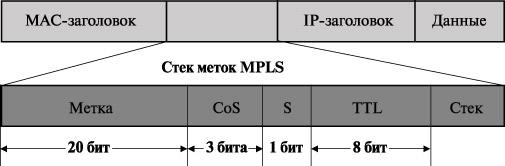
\includegraphics[scale=0.5]{pictures/mpls_label}
\caption{Структура MPLS метки}
\label{pic:mpls_label}
\end{figure}

Размер метки 4 байта. Она состоит из следующих полей:
\begin{itemize}
\item метка (LABEL), размер поля - 20 бит, используется для определения LSP;
\item класс сервиса (Class Of Service, CoS), размер поля - 3 бита, используется для реализации механизмов качества обслуживания и явного уведомления о перегрузке;
\item дно стека (Bottom Of Stack, S), размер поля - 1 бит, если флаг установлен, это означает, что данная метка является последней в стеке;
\item время жизни (Time To Live, TTL), размер поля - 8 бит, используется для предотвращения петель, как и в IP;
\end{itemize}

Распределение меток между LSR приводит к установлению внутри домена MPLS путей с коммутацией по меткам - LSP. Обмен метками между LSR осуществляется с использованием LDP, а также с помощью модифицированных версий других протоколов сигнализации в сети. Каждый маршрутизатор LSR содержит таблицу, которая ставит в соответствие паре "входной интерфейс, входная метка" тройку "префикс адреса получателя, выходной интерфейс, выходная метка". Получая пакет, LSR по номеру интерфейса, на который пришел пакет, и по значению метки определяет для него выходной интерфейс. Старое значение метки заменяется новым и пакет отправляется следующему устройству на пути LSP.

Вся операция требует лишь одноразовой идентификации значений полей в одной строке таблицы. Это занимает гораздо меньше времени, чем сравнение IP-адреса отправителя с наиболее длинным адресным префиксом в таблице маршрутизации, используемой при традиционном подходе.

Сеть MPLS делится на две функционально различные области - ядро и граничную область (рисунок~\ref{pic:mpls_net_example}). Ядро образуют устройства, минимальным требованием к которым является поддержка MPLS и участие в процессе маршрутизации трафика. Маршрутизаторы ядра занимаются только коммутацией. Все функции классификации пакетов по различным FEC, а также реализацию таких дополнительных сервисов, как фильтрация, явная маршрутизация, выравнивание нагрузки и управление трафиком берут на себя граничные LSR.  В результате, интенсивные вычисления приходятся на граничную область, а высокопроизводительная коммутация выполняется в ядре.
\begin{figure}
\centering
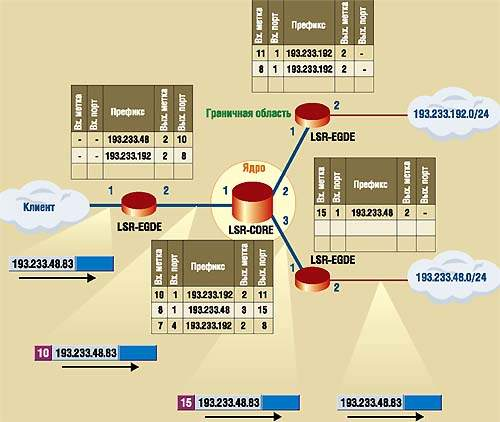
\includegraphics[scale=0.55]{pictures/mpls_net_example}
\caption{Схема коммутации MPLS}
\label{pic:mpls_net_example}
\end{figure}

На граничных маршрутизаторах может быть реализована классификация трафика с использованием технологии DPI. Такой подход придаст сети большую гибкость, гарантируя наиболее приоритетному трафику лучшие LSP.

Разрабатываемый сервис будет работать в MPLS сетях, выполняя функции граничного маршрутизатора.

\subsection{VLAN сети}
Коммутатор позволяет локализовать потоки информации, а также контролировать эти потоки и управлять ими с помощью механизма пользовательских фильтров. Однако такой фильтр способен воспрепятствовать передаче кадров лишь по конкретным адресам, тогда как широковещательный трафик он передает всем сегментами сети. Таков принцип действия реализованного в коммутаторе алгоритма моста, поэтому сети, созданные на основе мостов и коммутаторов, иногда называют плоскими - из-за отсутствия барьеров на пути широковещательного трафика.

VLAN позволяет преодолеть указанное ограничение, создавая виртуальную сеть - группа узлов сети, трафик которой, в том числе и широковещательный, на канальном уровне полностью изолирован от других узлов (рисунок~\ref{pic:vlan_net_example}). VLAN - это логический канал внутри физического.
\begin{figure}
\centering
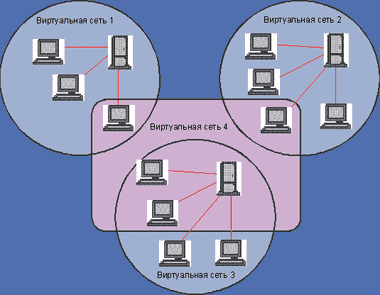
\includegraphics[scale=0.55]{pictures/vlan_net_example}
\caption{VLAN сеть}
\label{pic:vlan_net_example}
\end{figure}

Сеть любого крупного предприятия, а тем более провайдера, не может функционировать без применения VLAN, поскольку объемы данных колоссальны. Применение данной технологии дает следующие преимущества:
\begin{itemize}
\item группирование устройств по функционированию;
\item уменьшение количества широковещательного трафика в сети;
\item увеличение безопасности сети;
\item увеличение управляемости сети;
\end{itemize}

Традиционно разделение сети на виртуальные сегменты выполняется по следующим критериям:
\begin{itemize}
\item по порту;
\item по mac-адресу;
\item по протоколу;
\end{itemize}

В данной работе интерес представляет разделение на сегменты по протоколу. Обычно производится по данным сетевого (IP) и транспортного уровня (TCP/UDP), что лишает провайдеров возможности использовать протоколы более высоких уровней для классификации трафика и его последующей обработки. Разрабатываемый сервис будет работать во VLAN сетях, предоставляя возможность тегирования определенного трафика (добавление метки пакету).

В данной реализации метка будет присваиваться в зависимости от того, к какому протоколу принадлежит пакет. На рисунке~\ref{pic:vlan_tag} показана структура метки согласно IEEE 802.1Q - стандарта, описывающего процедуру тегирования трафика для передачи информации о принадлежности к VLAN.
\begin{figure}
\centering
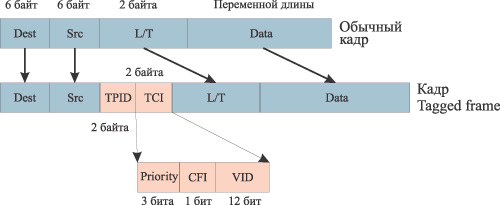
\includegraphics[scale=0.55]{pictures/vlan_tag}
\caption{VLAN метка}
\label{pic:vlan_tag}
\end{figure}

Размер тега - 4 байта. Он состоит из следующих полей:
\begin{itemize}
\item идентификатор протокола тегирования (Tag Protocol Identifier, TPID), размер поля - 16 бит, указывает какой протокол используется для тегирования, для 802.1Q используется значение 0x8100;
\item приоритет (Priority, PCP), размер поля - 3 бита, используется стандартом IEEE 802.1P для задания приоритета передаваемого трафика;
\item идентификатор канонического формата (Canonical Format Idicator, CFI), размер поля - 1 бит, указывает на формат mac-адреса, используется для совместимости между сетями Ethernet и Token Ring;
\item идентификатор VLAN (VLAN Identifier, VID), размер поля - 12 бит, указывает какому сегменту виртуальной сети принадлежит пакет, диапазон возможных значений от 0 до 4095;
\end{itemize}

Теоретический предел идентификаторов виртуальных сетей равен 4095 - на сегодняшний день этого недостаточно. Для решения этой проблемы используют технологию QinQ (стандарт IEEE 802.1AD), которая позволяет использовать внутри пакета две метки. Это расширяет количество идентификаторов до 16777216. Вторая метка имеет такую же структуру, как и первая, единственное отличие в значении поля TPID - в случае 802.1AD используется 0x88A8.


\section{Обзор существующих решений}
Системы DPI приобретают все большую популярность, несмотря на высокую стоимость. Сейчас почти у каждого большого вендора есть свое решение. У Cisco это Cisco SCE, у Huawei - SIG9800, у Juniper - VXA. Есть и менее известные компании, которые производят преимущественно оборудование DPI, например Allot или Inline Telecom.

Все эти решения являются сложными аппаратно-программными комплексами, поэтому не представляют большого интереса в рамках данной работы. Далее рассмотрены чисто программные решения, функциональные возможности  и цели которых схожи с разрабатываемым сервисом.
\subsection{Проект OpenDPI}
OpenDPI - библиотека для классификации сетевого трафика на основе технологии глубокого анализа пакетов. Она является свободной и распространяется под лицензией LGPLv3.

OpenDPI построен на базе продукта PACE, который разрабатывается компанией Ipoque, заимствовав многие особенности оттуда. Сам проект PACE является коммерческим и в рамках данной работы не рассматривается.

Основные особенности:
\begin{itemize}
\item не требует наложений патчей на ядро и iptables;
\item работает в виде модуля ядра и использует библиотеку xtables для внутренних нужд;
\item написан полностью на C, что повышает производительность;
\item для обнаружения используются модули, написанные на C, а не список регулярных выражений;
\item последняя версия библиотеки (v3.10, 2012 год) поддерживала порядка 100 протоколов;
\end{itemize}

В данный момент проект OpenDPI не поддерживается.

\subsection{Проект nDPI}
nDPI - библиотека, основанная на OpenDPI, поддерживаемая компаний ntop~\cite{ntop_company}. Это мощное DPI-решение, которое постоянно дорабатывается и улучшается и, на сегодняшний день, является самым продвинутым программным решением DPI для архитектуры x86\_64.

Основные особенности:
\begin{itemize}
\item не требует наложений патчей на ядро;
\item библиотека написана на языке C, что повышает производительность;
\item для обнаружения используются как модули на языке C, так и описание протокола в виде файла определенной структуры;
\item поддерживается более 150 протоколов, список которых постоянно пополняется;
\item работает под Linux и Windows;
\end{itemize}

Сама по себе библиотека nDPI предоставляет API для разработки конкретных сетевых приложений. Так она используется в других продуктах компании, например приложениях ntopng и nProbe. Поэтому рассматривать nDPI как прямой аналог разрабатываемого сервиса нельзя.


\section{Быстрая обработка пакетов}
Разрабатываемый сервис должен иметь высокие показатели производительности. Этого нельзя добиться просто используя более быстрый чип на сетевой карте, требуется использовать все возможности современных вычислительных систем, а также различные техники ускорения обработки.

\subsection{Возможности вычислительных систем}
\paragraph{Кэши}

На рисунке~\ref{pic:memory_schema} показаны различные уровни памяти современных CPU и примерное время доступа к ним. Такая архитектура введена для того, чтобы минимизировать время доступа программ к данным. Чем выше по иерархии находятся необходимые данные, тем выше производительность приложения в целом.
\begin{figure}[h]
\centering
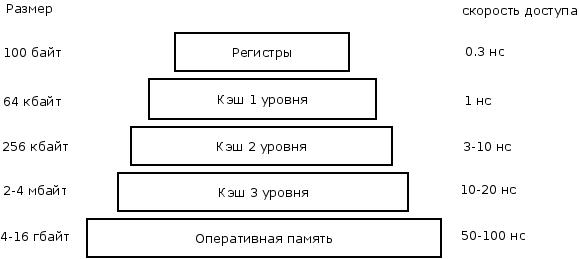
\includegraphics[scale=0.7]{pictures/memory_schema}
\caption{Иерархия памяти}
\label{pic:memory_schema}
\end{figure}

Для сокращения времени доступа к памяти данные могут быть помещены в кэш до того, как они действительно понадобятся. Такой подход реализуется как программно (software prefetching), так и на уровне железа (hardware prefetching).

\paragraph{TLB}

TLB~\cite{modern_os} представляет собой кэш ограниченного размера, хранящий отображение виртуальных адресов памяти в физические. При обращении к данным по виртуальному адресу просматриваются записи в TLB и, если нужная запись присутствует, возвращается физический адрес. В этом случае задержка несоизмеримо мала. В противном случае, когда нужной записи в кэше нет, требуется выполнять преобразование виртуального адреса в физический с последующим сохранением данных в TLB, что занимает несколько тактов процессора и негативно сказывается на производительности приложения, запросившего данные.

\paragraph{DMA}

DMA~\cite{modern_os} позволяет различным устройствам ввода-вывода обращаться к памяти напрямую, без привлечения центрального процессора. Однако, процессор должен подготовить для этого буфер в памяти и передать указатель на него устройству, которому необходим DMA, например сетевой карте. Таким образом, сетевая карта сможет считывать и записывать данные, используя этот буфер, вне зависимости от занятости процессора. Существует еще один подход под названием DCA. Он позволяет устройствам ввода-вывода записывать данные напрямую в кэш. Например, сетевая карта может помещать в кэш входящие пакеты, минуя оперативную память и не привлекая процессор.

Все это повышает скорость обработки за счет ликвидации копирования данных из памяти в процессор.

\paragraph{RSS}

Современные сетевые карты имеют несколько RX и TX очередей. Для утилизации всей пропускной способности сетевая карта может помещать пакеты в различные очереди, а каждая очередь может обрабатываться отдельным ядром процессора.

Для разделения пакетов по очередям используют подсчет хэша, соответственно трафик с одним значением хэша попадает в одну очередь, со вторым значением в другую. Такой подход позволяет масштабировать обработку данных, обрабатывая разные очереди на разных ядрах, тем самым повышая общую производительность системы.

\paragraph{Другие возможности}

Некоторые операции, такие как подсчет хэша и валидация контрольных сумм, могут быть реализованы в самих сетевых картах. Это делается для того, чтобы не нагружать процессор дополнительными вычислениями. Например, современные карты сами считают CRC для Ethernet кадров. Схожие возможности реализованы и для протоколов более высоких уровней, таких как IP и TCP/UDP.

\subsection{Техники ускорения обработки}
Фреймворки используют многочисленные техники ускорения. Некоторые их них совершенно новые в сфере обработки пакетов (не использовать стандартный сетевой стек, избегать копирования пакетов, выделять память заранее), а некоторые давно используются в современных операционных системах (режим опроса, обработка партиями).

\paragraph{Стандартный сетевой стек ядра}

Ядро выполняет большую работу по обработке трафика, анализируя пакеты, пропуская каждый из них через стек протоколов, на что тратится время. Основная задача фреймворков - как можно быстрее доставлять пакеты в режим пользователя, в котором уже реализуется обработка трафика в соответствие с логикой разрабатываемого приложения. Поэтому дополнительная обработка пакетов ядром, которая, к тому же, требует большого количества времени, не имеет смысла.

\paragraph{Копирование пакетов}

При отправке пакета, используя традиционный интерфейс системы, пакет необходимо скопировать из пользовательского сокета в буфер ядра (или наоборот). Это вносит дополнительную задержку в обработку, которых стараются избегать фреймворки, выделяя для этого буфер в памяти, который используется и приложением пользователя, и обработчиками пакетов. Сетевая карта считывает/записывает данные из/в область памяти (через DMA), а приложение пользователя записывает/считывает данные из этой же области.

Время копирования пакета напрямую зависит от его длины, поэтому время пересылки коллекции пакетов из сетевой карты в определенную область памяти не является постоянной величиной и меняется, в зависимости от длины каждого пакета в коллекции.

Еще одно преимущество - это возможность легко реализовывать приложения пересылки данных. Для этого не нужно копировать полученные пакеты в какой-то буфер, используемый для последующей отправки. Достаточно пометить пакет как "готовый для отправки".

\paragraph{Преждевременное выделение памяти}

Выделение памяти осуществляется в ядре операционной системы. Это может быть необходимо, когда буфер для приема пакетов не имеет достаточную длину для сохранения вновь полученного пакета. Выделение памяти приводит к системному вызову, что вносят дополнительную задержку в обработку. Аналогичная ситуация с буфером для отправки пакетов.

В фреймворках быстрой обработки пакетов память, необходимая для работы, выделяется заранее, на этапе инициализации и запуска приложения. Это позволяет избежать частых системных вызовов, повысив общую производительность. Так как размер выделенной памяти не может быть изменен в режиме реального времени, он должен быть достаточным для всех нужд приложения.

\paragraph{Режим опроса}

Раньше обработка пакетов осуществлялась через прерывания - когда на сетевой карте появлялся новый пакет, происходило прерывание и ядро обрабатывало этот пакет. При высоких скоростях трафика  ядро не успевало обрабатывать все прерывания, из-за чего страдала производительность. В современных системах при высоких нагрузках происходит переключение режима обработки с прерываний на режим опроса (polling)~\cite{modern_os}, при котором в цикле выполняется опрос сетевой карты на предмет появления новых данных.

Такой подход реализован не только в современных ОС, но и в фреймворках быстрой обработки пакетов.

\paragraph{Большие страницы}

Для того, чтобы избежать промахов в TLB, могут использоваться большие страницы памяти (huge pages)~\cite{linux_programming}. Размер страницы, обычно, увеличивается с 4 Кбайт до 2 Мбайт. Все это приводит к минимизации времени доступа к данным, находящимся в больших страницах памяти.

Детально, увеличение размера страницы приводит к сокращению числа записей в TLB, например для последних процессоров Intel с 256 записей (4 КБайт) до 32 (2 Мбайта).

\paragraph{Обработка партиями}

Практически все фреймворки предоставляют API для получения пакетов с сетевой карты.  Каждый вызов функции требует определенного количества процессорного времени, поэтому требуется, по возможности, минимизировать количество таких вызовов. Это решается предоставлением такого API, который за один вызов получает не один пакет, а партию, тем самым разделив стоимость вызова на несколько пакетов сразу.

\subsection{{PF\_RING}}
Является одним из наиболее популярных фреймворков для обработки пакетов. В данный момент поддерживается компанией ntop, состоит из набора модулей. Модуль ядра PF\_RING и драйвера распространяются под лицензией GNU GPLv2, а библиотека для пространства пользователя под лицензией LGPLv2.1 и доступна в формате исходного кода. На рисунке~\ref{pic:pfring_example} показана концептуальная схема приложения, использующего PF\_RING.
\begin{figure}[h]
\centering
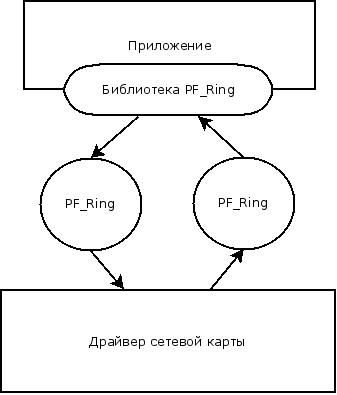
\includegraphics[scale=0.7]{pictures/pfring_example}
\caption{Использование PF\_RING}
\label{pic:pfring_example}
\end{figure}

Для получения высоких показателей производительности рекомендуется использовать улучшенную версию фреймворка - PF\_RING ZC (Zero Copy). Точная архитектура этой версии неизвестна, так как продукт является коммерческим. Согласно данным компании ntop, фреймворк основан на библиотеке libZero и его производительность - line rate на 10 Гбит/сек. Список поддерживаемых сетевых карт мал, так, например, для сетевых карт Intel доступны только драйвера e1000e, igb, ixgbe.

Основные особенности PF\_RING:
\begin{itemize}
\item использует большие страницы;
\item использует DMA;
\item использует прерывания только для выхода из заблокированного системного вызова, в остальном используется режим опроса;
\item предоставляет API для обработки партиями;
\item не использует системные вызовы для обработки пакетов;
\item не требует патчей на ядро, использует модули;
\end{itemize}

\subsection{DPDK}
Разработанный и поддерживаемый компанией Intel, фреймворк DPDK~\cite{dpdk_descr} является наиболее популярным и привлекательным для применения в разработке различных сетевых приложений. Строго говоря, DPDK - это набор программных библиотек, которые могут улучшить производительность при обработке пакетов. Является полностью свободным программным обеспечением и распространяется под лицензией Open Source BSD.

Основная цель DPDK не просто ускорить обработку пакетов, но и предоставить набор полезных библиотек, которые позволят разработчикам создавать собственные сетевые приложения. На рисунке~\ref{pic:dpdk_eal} приведены основные библиотеки DPDK с наиболее значимой библиотекой, называемой Environment Abstraction Layer (rte\_eal).
\begin{figure}
\centering
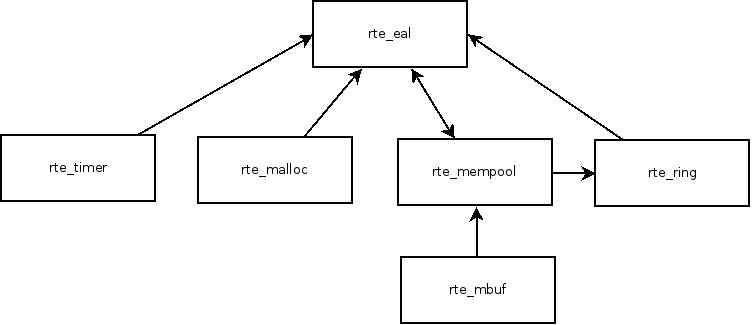
\includegraphics[scale=0.5]{pictures/dpdk_eal}
\caption{Основные библиотеки DPDK}
\label{pic:dpdk_eal}
\end{figure}

Главная библиотека rte\_eal используется для того, чтобы скрыть детали реализации на уровне железа и операционной системы от приложения пользователя и других библиотек. В этой библиотеке реализована инициализация всех ресурсов, таких как память, таймеры и компоненты шины данных. Использование библиотеки rte\_timer позволяет вызывать функции асинхронно, один раз или периодически. Точное начало отсчета времени обеспечивается через EAL. Компонент rte\_malloc используется для выделения памяти в больших страницах для использования памяти более эффективно. Библиотека rte\_mbuf предоставляет буфера для хранения пакетов, которые могут адаптироваться для хранения любых данных. Все буфера создаются при запуске приложения. rte\_ring предоставляет буфера фиксированного размера, основная особенность которых состоит в том, что они реализуют идеологию lock free, т.е. одновременно несколько потоков могут писать в буфер и читать из него. Используются для быстрого взаимодействия между различными потоками. rte\_mempool используется для сохранения объектов.

Все это лишь малая часть библиотек, поставляемых DPDK. Доступны такие библиотеки, как rte\_hash для вычисления хэша, rte\_cofig для удобного описания и парсинга конфигураций и многие другие.

DPDK предоставляет большой список драйверов для физических и виртуальных интерфейсов. Для того, чтобы использовать эти драйвера, необходимо привязать сетевую карту к нужному драйверу. Ядро Linux не имеет доступа к устройству, пока его обслуживает драйвер DPDK. Ниже представлен неполный список доступных драйверов:
\begin{itemize}
\item xenvirt
\item vmxnet3
\item virtio
\item ixgbe
\item i40e
\item e1000
\end{itemize}

Основные особенности DPDK:
\begin{itemize}
\item использует большие страницы;
\item использует DMA;
\item не использует прерывания, только режим опроса;
\item не использует системные вызовы;
\item не требует патчей на ядро, в основном используется модуль igb\_uio;
\item большой набор поддерживаемых сетевых карт;
\item высокие показатели производительности (10 Гбит/сек на 1 ядре);
\item широкий набор дополнительных библиотек;
\item API для обработки пакетами;
\end{itemize}

\section{Постановка задачи}
Учитывая все проблемы интернет-провайдеров, описанные выше, а также проанализировав технологию DPI и доступные фреймворки быстрой обработки пакетов, необходимо реализовать сетевой сервис классификации трафика на основе технологии DPI, который должен:
\begin{itemize}
\item работать с любыми Ethernet картами, поддерживаемыми DPDK;
\item автоматически определять нужный драйвер;
\item выполнять функцию сетевого экрана;
\item выполнять функцию граничного маршрутизатора в MPLS сети;
\item выполнять тегирование трафика согласно 802.1Q и 802.1AD;
\item поддерживать конфигурирование на каждый порт;
\item использовать фреймворк DPDK и все его потенциальные возможности;
\item собирать статистику по каждому протоколу;
\end{itemize}

Разрабатываемый сервис должен быть полностью законченным приложением, а не отдельной библиотекой, предоставляющей API, а также должен быть покрыт модульными тестами. Поддерживаемые протоколы:
\begin{itemize}
\item HTTP;
\item SIP;
\item RTSP;
\item RTP;
\end{itemize}

На вход данного сервиса допускается только Ethernet/IP/TCP(UDP) трафик, который может быть тегированным. Все остальные виды трафика будут блокироваться.

\paragraph{Выводы}

В рамках данного раздела были изучены возможные варианты применения технологии DPI в сетях интернет-провайдеров. Рассмотрены случаи использования сервиса на основе DPI в качестве межсетевого экрана, граничного маршрутизатора в MPLS сетях, а так же возможность его использования для тегирования трафика. Для увеличения производительности были приведены некоторые техники ускорения, а также проанализированы фреймворки быстрой обработки пакетов. В конце раздела представлен полный список требований к разрабатываемому сервису.
